% paper_en.tex -- compile with XeLaTeX, Biber, XeLaTeX x2
\documentclass[11pt,a4paper]{article}
% ---------- shared preamble for paper_en.tex and paper_vi.tex ----------
\usepackage{fontspec}
\IfFontExistsTF{Times New Roman}{\setmainfont{Times New Roman}}{\setmainfont{TeX Gyre Termes}}
\usepackage{geometry}
\geometry{left=2.5cm,right=2.5cm,top=2.5cm,bottom=2.5cm}
\usepackage{setspace}
\onehalfspacing
\usepackage[table]{xcolor}
\definecolor{ndblue}{RGB}{12,35,64}
\usepackage{graphicx}
\graphicspath{{figures/}}
\usepackage{booktabs,tabularx,array,multirow,longtable,threeparttable}
\usepackage{amsmath,amssymb,bm}
\usepackage{csquotes}
\usepackage{float}
\usepackage{enumitem}
\setlist{itemsep=2pt,topsep=3pt}
\usepackage{caption}
\captionsetup{font=small,labelfont=bf,justification=justified,singlelinecheck=false}
\usepackage{titlesec}
\titleformat{\section}{\bfseries\large}{\thesection.}{0.5em}{}
\titleformat{\subsection}{\bfseries\normalsize}{\thesubsection.}{0.5em}{}
\titleformat{\subsubsection}{\itshape\normalsize}{\thesubsubsection.}{0.5em}{}
\usepackage{xurl}
\usepackage{float}
\usepackage[colorlinks=true,linkcolor=ndblue,citecolor=ndblue,urlcolor=ndblue]{hyperref}
\newcolumntype{Y}{>{\raggedright\arraybackslash}X}
\newcommand{\EV}{\mathbb{E}}
\newcommand{\srcnote}[1]{{\footnotesize\textit{#1}}}

\usepackage[english]{babel}
\usepackage[backend=biber,style=apa,sorting=nyt,maxcitenames=2,maxbibnames=20,doi=true,url=false,isbn=false]{biblatex}
\DeclareLanguageMapping{english}{english-apa}
\addbibresource{references.bib}
\AtEveryBibitem{\clearfield{note}}
\AtBeginBibliography{\small\sloppy}

\title{\textbf{Why Subsidised Aquaculture Insurance Does Not Reach Farmers: Climate Hazards, Trigger Design and Risk-Based Pricing in Vietnam's Mekong Delta}}
\author{Truong Nhat Duy}
\date{October 2026}

\setlength{\emergencystretch}{3em} % tránh dòng tràn lề (13/10/2026)
\begin{document}
\maketitle

\begin{abstract}
\noindent Vietnam subsidises up to 90\% of agricultural insurance premiums for poor and near-poor households and 20\% for others, and since 2019 has targeted shrimp (since 2022 also pangasius) in the five coastal Mekong Delta provinces that produce 73\% of its farmed shrimp. A 2026 decree raises the caps to 95\%, 50\% and 30\%. This paper asks why subsidised insurance has almost never reached fish and shrimp farmers. I combine twelve rounds of the Vietnam Household Living Standards Survey (2002--2024; 21,726 aquaculture household-rounds in coastal and Mekong provinces), its commune disaster module, district-level gridded climate data, cyclone tracks, satellite sea-surface temperature and a 2005--2024 provincial production panel. Five findings emerge. First, the first stage is essentially zero: in every round, 0--1\% of fish-farming households in the pilot provinces received an insurance payout, with no break after the policy. Second, the legal peril list covers salinity intrusion, heat and drought, but pays only after an official disaster declaration and excludes disease. Third, synthetic difference-in-differences estimates of programme effects on provincial output are close to zero (0.016, SE 0.066) and rule out effects above about 18\%. Fourth, gridded hazard indices neither predict household output nor identify which communes report a disaster: within province-year, the area under the ROC curve is 0.47--0.51 for drought and 0.56--0.63 for floods, implying large basis risk for weather-index products. Fifth, land-based hazards show no robust trend over 1991--2024, but marine-heatwave days in the pilot provinces' coastal waters rose from about 7 to 53 a year between 1999--2009 and 2015--2024, so historical climatologies understate current heat exposure. The binding constraints are trigger design, data and supply, not the subsidy rate.

\medskip
\noindent\textbf{Keywords:} agricultural insurance; aquaculture; take-up; adverse selection; charity hazard; basis risk; credibility theory; marine heatwaves; Mekong Delta; Vietnam.\\
\noindent\textbf{JEL:} Q14, Q22, Q54, G22, H23, O13.
\end{abstract}

\clearpage
%====================================================================
\section{Introduction}
\label{sec:intro}

Aquaculture is one of the fastest-growing food sectors in the world and one of the most exposed to climate hazards. Vietnam ranks among the largest producers of farmed aquatic animals, and in 2024 its 13 Mekong Delta provinces accounted for 71.9\% of national aquaculture output \parencite{nso_pxweb,fao_fishstat2026}. Shrimp is even more concentrated: five coastal provinces (Bến Tre, Trà Vinh, Sóc Trăng, Bạc Liêu and Cà Mau) produced 1.03 of the country's 1.41 million tonnes of farmed shrimp. These are the only provinces where shrimp insurance premiums have been subsidised since 2019 \parencite{decision22_2019,decision13_2022}.

Public subsidies for agricultural insurance are widespread in developing countries, but their record is mixed. Multi-peril schemes run or subsidised by the state have often produced high loss ratios and fiscal pressure \parencite{hazell1992,mahul2010}, while index insurance, the main alternative, suffers from low demand even when heavily subsidised, largely because of basis risk and limited trust \parencite{carter2017,jensen2017,cole2013,clarke2016}. Evidence on aquaculture is particularly thin: reviews by FAO note that insurance schemes in Asia generally do not serve small-scale producers and that insurers remain uncertain about the viability of the line \parencite{vananrooy2006,secretan2007}.

This paper studies Vietnam's subsidised shrimp insurance programme and asks why it has failed to reach farmers. The question matters because Decree 346/2026/ND-CP, effective 20 October 2026, raises premium subsidy caps to 95\% for poor and near-poor households, 50\% for other households and 30\% for eligible organisations, and devolves to provincial People's Councils the choice of areas, insured objects, perils and subsidy levels \parencite{decree346_2026,tckttc2026nd346}. If low coverage stems from the price farmers pay, higher subsidies are the right response. If it stems from contract design, trigger rules, missing data or insurers' unwillingness to supply, higher subsidies alone will not work.

I combine five types of data: twelve rounds of the Vietnam Household Living Standards Survey (VHLSS) from 2002 to 2024, harmonised at the household level; district-level gridded climate data (CHIRPS rainfall, NASA POWER temperature, SPEI drought indices) for 1991--2024; cyclone wind fields reconstructed from IBTrACS; satellite sea-surface temperature for coastal waters; and a provincial production panel for 2005--2024. I also verify the legal texts directly, including an optical-character-recognition reading of the signed Decision 22/2019/QD-TTg, and compile the administrative figures released by the Ministry of Finance.

The paper establishes five findings. \textit{First}, the first stage is essentially zero. In every VHLSS round from 2004 to 2024, between 0 and 1\% of fish-farming households in the pilot provinces received an insurance payout, and the share shows no break after June 2019 or June 2022. Ministry of Finance figures reported in the press tell the same story: between 2019 and early 2025, only four of 29 eligible localities implemented the subsidy, all for rice or cattle \parencite{tbtc2025nd58}. \textit{Second}, the reason is not that the legal peril list ignores the Delta's hazards. Article 5 of Decision 22/2019 covers salinity intrusion, heat and drought for shrimp, but only when the disaster is ``announced or confirmed by a competent state authority''; disease is excluded. \textit{Third}, synthetic difference-in-differences (SDID) estimates of the effect on provincial output are near zero and, given the minimum detectable effect, rule out effects on total output above roughly 18\%. The apparent positive effect on shrimp is matched by a placebo that assigns the policy to 2015. \textit{Fourth}, gridded wet and dry-hot hazard indices do not predict household aquaculture output once commune and province-by-year fixed effects are included, and they barely distinguish communes that report a drought or flood from those that do not. Both results imply large basis risk for weather-index insurance. \textit{Fifth}, the hazards that gridded indices measure on land show no robust trend over 1991--2024, whereas heat in the coastal waters of the pilot provinces has risen sharply; province-level premium differences are mostly sampling noise, and an equilibrium simulation with assumed parameters suggests that better risk information raises coverage at lower fiscal cost than flat subsidy increases.

The paper contributes to three literatures. It adds to the economics of agricultural insurance in developing countries \parencite{hazell1992,just1999,carter2017,jensen2016} by documenting a near-zero first stage over two decades in a nationally representative sample, and by showing that the binding constraint in this setting is trigger design and supply rather than price. It contributes to the small literature on aquaculture insurance \parencite{vananrooy2006,secretan2007,hobday2025} and to Vietnamese studies of insurance demand, which rely on stated preferences in one or two provinces \parencite{khoi2014tom,nghi2016tom,nguyenkat2021,tu2025}. And it adds to the household-level evidence on natural disasters in Vietnam \parencite{thomas2010,bui2014,arouri2015,hoang2024} by separating aquaculture households and by using physical hazard measures rather than self-reported events. Finally, it offers a simple test of basis risk that uses the disaster reports of local officials as a benchmark for gridded indices, a check that can be replicated wherever household surveys include a community module.

Section~\ref{sec:lit} reviews the related literature. Section~\ref{sec:background} describes the institutional setting. Section~\ref{sec:framework} sets out a simple framework. Section~\ref{sec:data} describes the data and Section~\ref{sec:strategy} the empirical strategy. Section~\ref{sec:results} presents results, Section~\ref{sec:discussion} discusses mechanisms and limitations, and Section~\ref{sec:policy} draws policy implications.

\section{Related literature}
\label{sec:lit}

\textit{Why insurance markets for disaster risk fail.} Four market failures are relevant. First, farmers know more about their own risk than insurers do, and a premium that does not reflect this drives low-risk buyers out \parencite{akerlof1970,rothschild1976}. \textcite{einav2011} show that the resulting equilibrium covers fewer people than is efficient, and \textcite{crocker1986} show that classifying risks on observable characteristics, combined with suitable transfers, can be Pareto improving. This is the theoretical case for risk-zoned premiums with progressive subsidies. Second, disaster losses are covariate within a region. Village risk sharing handles idiosyncratic shocks well but not common ones \parencite{townsend1994,dercon2002}, and insurers must hold capital or buy reinsurance against the tail \parencite{kunreuther1996}. Third, risk information such as hazard maps and loss histories has the features of a public good. \textcite{mendelsohn2000} argues that most adaptation is private and will be undertaken efficiently by private agents, but that the public role lies in public goods, including information. Fourth, governments cannot commit to withholding relief. \textcite{coate1995} shows that altruistic relief to the uninsured leads the poor to underinsure, and \textcite{clarkedercon2016} argue for pre-arranged disaster finance with explicit payout rules. \textcite{furton2019} suggest reading both kinds of failure as institutional mismatch, in which the rules that govern interaction do not fit the problem agents face; trigger rules and peril lists are such rules. Subsidies can themselves create a policy failure: in the United States they have tilted land use and crop choice towards riskier production \parencite{goodwin2013}.

\textit{The low-demand puzzle.} Reviews conclude that demand for agricultural insurance in developing countries is low at actuarially fair or commercial prices and that index products have not reached scale without heavy subsidy \parencite{colexiong2017,carter2017}. Experiments point to barriers beyond price. In India, take-up of rainfall insurance falls with basis risk, rises with wealth and is lower among credit-constrained households, while more risk-averse households buy less, not more \parencite{gine2008}. Trust in and familiarity with the provider, and information shared through social networks, raise take-up \parencite{gine2008,cai2015}. Liquidity matters: allowing Kenyan farmers to pay the premium at harvest raised take-up from 5\% to 72\% \parencite{casaburi2018}. Basis risk can make index insurance unattractive to the most risk-averse \parencite{clarke2016}, and is large and heterogeneous in practice \parencite{jensen2016}. Informal risk sharing can complement index insurance when basis risk is idiosyncratic \parencite{mobarak2013}, and the value of index insurance is greatest when it is interlinked with credit \parencite{carter2016}. \textcite{binswanger2012} argues that better-off farmers already self-insure while the poorest cannot afford upfront premiums. These findings matter for shrimp farming, where up-front input costs are high and premiums compete with seed and feed for scarce cash.

\textit{Charity hazard and recovery.} Expected public relief lowers flood insurance purchase among German homeowners \parencite{andor2020}, and post-disaster federal grants reduce subsequent flood insurance coverage in the United States \parencite{kousky2018}. Insurance is associated with faster recovery, but its signalling role is weakened when premiums do not reflect risk \parencite{kousky2019}. All of this evidence comes from high-income countries; I am not aware of comparable estimates for subsidised agricultural insurance in a developing country.

\textit{Aquaculture.} Surveys of aquaculture producers find that price and disease risks rank above weather risks in Norway \parencite{bergfjord2009}, among shrimp farmers in Bangladesh \parencite{ahsan2011} and among pangasius farmers in the Mekong Delta \parencite{lecheong2010}. These are the risks that the Vietnamese product excludes. FAO reviews note that existing schemes in Asia rarely serve small-scale farmers \parencite{vananrooy2006,secretan2007}, and parametric products based on ocean indicators face basis risk and cost constraints \parencite{hobday2025}.

\textit{Changing hazards.} Marine heatwaves have become longer and more frequent globally: between 1925 and 2016 their average frequency rose by 34\%, their duration by 17\% and the number of marine heatwave days per year by 54\%, largely because of rising mean ocean temperatures \parencite{oliver2018}. They are projected to increase sharply with further warming \parencite{frolicher2018}. In the Mekong Delta, tidal amplitude inside the delta is rising by about 2 cm per year and channel salinity by 0.2--0.5 PSU per year, far faster than sea-level rise alone would imply; \textcite{eslami2019} attribute this to 2--3 m of riverbed incision caused by reduced upstream sediment supply and sand mining, so salinity risk is partly human-made and non-stationary. Both strands suggest that historical loss distributions may understate future risk, whereas experience-based rating assumes that the past is representative. Methodologically, I follow the climate-econometrics practice of identifying weather effects from within-unit variation \parencite{dell2014,hsiang2016}, and distinguish asset losses from welfare losses as in \textcite{hallegatte2017}.

%====================================================================
\section{Institutional background}
\label{sec:background}

\subsection{The sector}

Viet Nam is the world's fourth-largest producer of farmed aquatic animals by quantity and the third-largest by value (Figure~\ref{fig:world}). In 2024 it produced 5.64 million tonnes live weight, 5.5\% of world output, worth 16.7 billion US dollars at current prices, 4.5\% of world value \parencite{fao_fishstat2026}. Its weight is much larger in the species that the subsidised insurance covers: Viet Nam produced 59\% of the world's farmed striped catfish (pangasius), 35\% of giant tiger prawn and 12\% of whiteleg shrimp, and these three species made up 68\% of the value of its aquaculture.

Growth has been fast but is slowing (Figure~\ref{fig:growth}a). Output grew by 13.5\% a year in 1994--2004, 10.8\% in 2004--2014 and 5.4\% in 2014--2024, against 7.2\%, 5.3\% and 3.8\% for the world; in value terms Viet Nam grew faster than the world in the first and last decades but not in 2004--2014, when Chinese aquaculture value rose by 16\% a year. Since the mid-2010s shrimp, above all whiteleg shrimp, has overtaken pangasius as the main source of value: in 2024 whiteleg shrimp was worth 5.8 billion US dollars, giant tiger prawn 2.7 billion and pangasius 2.9 billion (Figure~\ref{fig:growth}c). National statistics show how the growth was achieved: between 1995 and 2024 output rose about 15-fold while harvested area rose 2.5-fold, so output per hectare rose from 0.86 to 5.26 tonnes \parencite{nso_pxweb}. Growth has thus come mainly from intensification, which concentrates more value in each hectare of pond exposed to the hazards discussed below. FAO and NSO totals differ slightly (5.64 and 5.90 million tonnes in 2024); I use FAO for international comparisons and NSO for domestic series.

\begin{figure}[htbp]
\centering
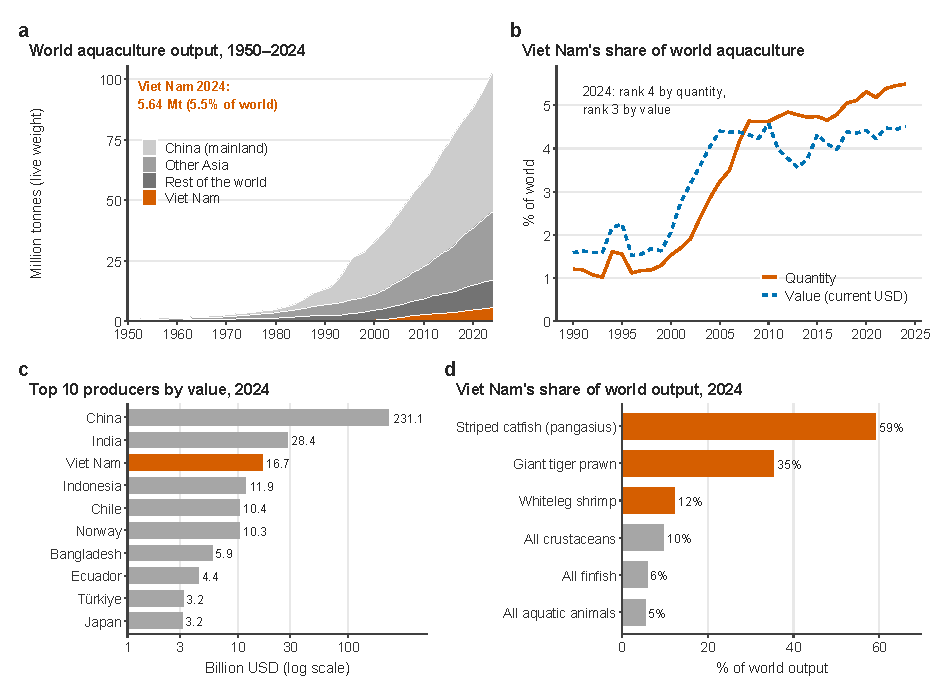
\includegraphics[width=160mm]{jf11_world_aquaculture.pdf}
\caption{Viet Nam in world aquaculture. (a) World aquaculture output of aquatic animals by producer group, 1950--2024; ``Other Asia'' excludes mainland China and Viet Nam. (b) Viet Nam's share of world output by quantity and by value (current USD), 1990--2024. (c) The ten largest producers by value in 2024 (log scale). (d) Viet Nam's share of world output in 2024 for the three species covered by subsidised insurance (orange) and for broad groups. Aquatic plants are excluded throughout. \textit{Source:} FAO FishStat, global aquaculture production 1950--2024 (release 2026.1.0); author's calculations.}
\label{fig:world}
\end{figure}

\begin{figure}[htbp]
\centering
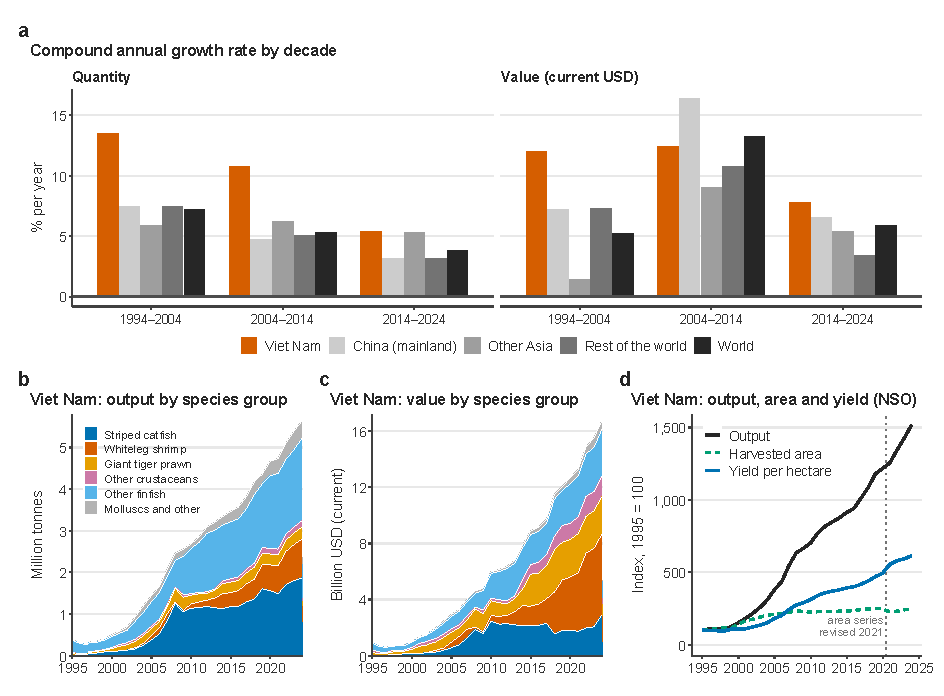
\includegraphics[width=160mm]{jf12_sector_growth.pdf}
\caption{Growth of aquaculture in Viet Nam and the world. (a) Compound annual growth rate of output quantity and value by producer group over three decades. (b, c) Viet Nam's aquaculture output and value by species group, 1995--2024. (d) National output, harvested area and output per hectare, index 1995 = 100; the harvested-area series is revised from 2021 (dotted line), so the change in area and yield between 2020 and 2021 is not comparable. Values are in current US dollars and include price changes. \textit{Source:} FAO FishStat 2026.1.0 (a--c); NSO PX-Web tables V06.58 and V06.68 (d); author's calculations.}
\label{fig:growth}
\end{figure}

\subsection{The legal framework}

Agricultural insurance in Vietnam was piloted under Decision 315/QD-TTg of 1 March 2011 for 2011--2013 in 20 provinces, covering rice, livestock and aquaculture \parencite{decision315_2011}. According to Ministry of Finance figures reported in the press, 7,487 households bought shrimp and fish insurance during the pilot, paying 218.1 billion VND in premiums, while claims reached 675.9 billion VND, about 3.1 times premiums; foreign reinsurers declined to take on shrimp and fish risks \parencite{tbtc2016bhts}. Aquaculture was not continued after the pilot.

Decree 58/2018/ND-CP set the permanent framework. Article 19 caps premium support at 90\% for individuals in poor and near-poor households and 20\% for other individuals and eligible organisations; Article 20 lists the natural disasters and diseases that may be supported; Article 3 already allows indemnity, yield, weather-index and remote-sensing-index products \parencite{decree58_2018}. The Prime Minister then specifies objects, perils, areas and periods. Decision 22/2019/QD-TTg (26 June 2019) supported tiger and whiteleg shrimp in the five provinces until 31 December 2020; Decision 03/2021/QD-TTg extended it to the end of 2021 and updated the poverty standard; Decision 13/2022/QD-TTg covered 24 June 2022 to 31 December 2025 and added pangasius \parencite{decision22_2019,decision03_2021,decision13_2022,tbtc2022qd13}. Decree 346/2026/ND-CP, signed on 5 September 2026, raises the caps to 95/50/30\% and devolves design choices to provincial People's Councils \parencite{decree346_2026,tckttc2026nd346}.

\subsection{Perils and triggers}

The peril list matters for the argument. I read the signed text of Decision 22/2019 directly. Article 5(3) lists the natural disasters supported for shrimp: storms, tropical depressions, whirlwinds, lightning, heavy rain, floods, inundation, landslides and subsidence caused by rain or flow, storm surge, \emph{salinity intrusion, heat waves, drought}, hail, earthquakes and tsunamis. Two conditions follow: disasters ``must be announced or confirmed by a competent state authority'', and ``disease risks are not supported'' for shrimp. Decision 13/2022 keeps the same list for shrimp and pangasius \parencite{tbtc2022qd13}. The product is often described as covering mainly storms and floods; the legal text does not support that reading. The relevant mismatch is in the trigger rule and the disease exclusion, not in the list of perils.

\subsection{Implementation}

Administrative figures are available only through press reports of Ministry of Finance statements. From 2019 to early 2025, four of 29 eligible localities implemented the subsidy: Nghệ An and Thái Bình for rice and Hà Giang and Bình Định for cattle. Across all objects, 20,261 households and organisations took part, with total premiums of 9.47 billion VND, of which 8.02 billion was paid by the state budget \parencite{tbtc2025nd58}. Under Decision 13/2022 the figure was 3,630 participants and 70.97 billion VND of insured value by early 2025; a later report gives 3,280 participants and 2.38 billion VND of premiums \parencite{baodautu2026bhnn,tbtc2026hangnghin}. None of these reports mentions a subsidised shrimp or pangasius contract. Officials cite missing loss data for rating, low subsidy levels, slow approval of beneficiary lists and the caution of international reinsurers \parencite{tbtc2025nd58,tbtc2026hangnghin}.

Figure~\ref{fig:context} places these instruments against the growth of the sector. Aquaculture output, summed over provinces, roughly quadrupled between 2005 and 2024, and the five pilot provinces accounted for about three-quarters of the increase in farmed shrimp. The subsidised shrimp product was in force for about six years between mid-2019 and the end of 2025, with a gap in the first half of 2022.

\begin{figure}[htbp]
\centering
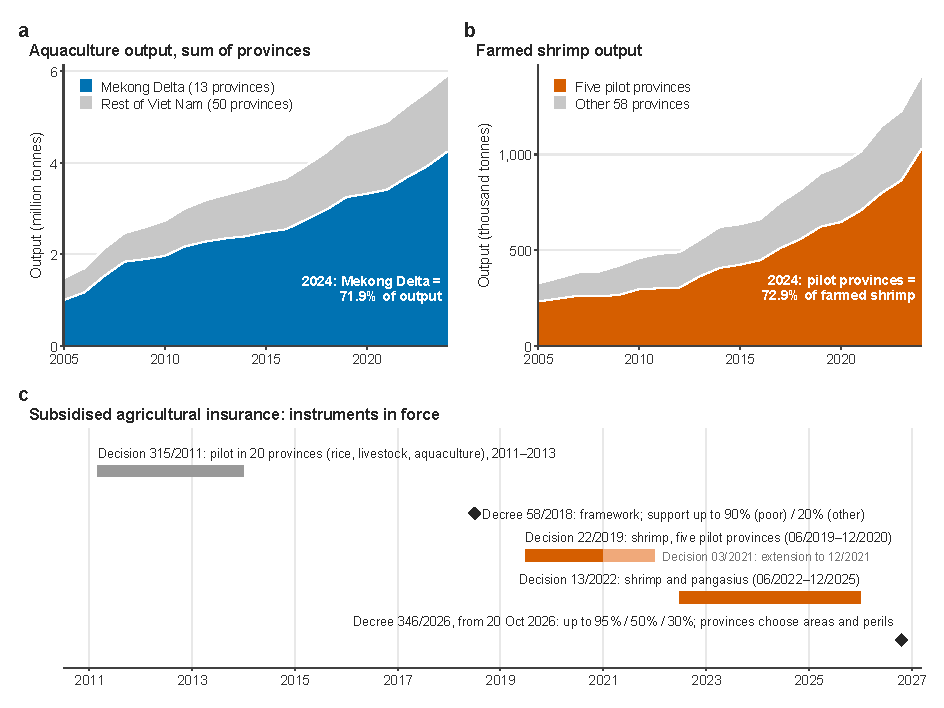
\includegraphics[width=160mm]{jf01_production_policy_timeline.pdf}
\caption{Aquaculture output and the subsidised insurance instruments. (a) Aquaculture output, Mekong Delta (13 provinces) and the rest of Viet Nam, sum of provincial figures. (b) Farmed shrimp output, five pilot provinces and the other 58 provinces. (c) Instruments in force; bars mark the periods stated in the legal texts, diamonds mark decrees whose effective dates within the year are not used in the analysis (Decree 58/2018) or fall after the data (Decree 346/2026). \textit{Source:} NSO PX-Web provincial tables; Decrees 58/2018 and 346/2026; Decisions 315/2011, 22/2019, 03/2021 and 13/2022.}
\label{fig:context}
\end{figure}

%====================================================================
\section{Conceptual framework}
\label{sec:framework}

\subsection{Demand with a trigger rule}

Let household $i$ in risk zone $z$ face a proportional loss $L_i$ on insured value $V$. Split the loss into a part caused by listed perils, $L^{c}_i$, and a part caused by unlisted risks such as disease, prices and management, $L^{u}_i$. Under the Vietnamese indemnity product the payout is
\begin{equation}
I_i = A_{zt}\,\max\big(L^{c}_i - d,\,0\big)\,V, \qquad \Pr(A_{zt} = 1 \mid H_{zt}) = \phi(H_{zt}),
\label{eq:trigger}
\end{equation}
where $d$ is the deductible and $A_{zt}$ indicates that a competent authority announces or confirms the disaster in zone $z$ and year $t$. A household with CRRA utility $u(\cdot)$, wealth $w$, premium $\pi_z$, subsidy rate $s_i$ and expected post-disaster relief $R_i$ buys insurance if
\begin{equation}
\EV\big[u(w - VL_i + I_i - (1-s_i)V\pi_z)\big] \geq \EV\big[u(w - VL_i + R_i)\big].
\label{eq:demand}
\end{equation}
Three features reduce the value of the contract regardless of $s_i$. When the unlisted share $\EV[L^{u}]/\EV[L]$ is large, the contract insures little of what farmers lose. When $\phi$ is low for chronic, local hazards such as salinity intrusion, the contract carries an ``administrative basis risk'' analogous to the basis risk of index products \parencite{clarke2016,jensen2016}. When relief $R_i$ is not netted against indemnities, insurance competes with free public cover \parencite{raschky2007,kousky2018}.

\subsection{Pricing and adverse selection}

An insurer that observes only a noisy signal of each household's risk type sets a break-even premium over the pool of buyers $B_z$:
\begin{equation}
\pi_z = (1+\theta)\,\EV[I_i \mid i \in B_z(\pi_z)] + \kappa\,\big(\mathrm{CVaR}_{q}(I_z) - \EV[I_z]\big),
\label{eq:premium}
\end{equation}
where $\theta$ is the loading and $\kappa$ the cost of capital for tail risk. With a uniform premium and heterogeneous private risk, low-risk households exit and the ratio $\EV[I \mid B]/\EV[I]$ exceeds one \parencite{rothschild1976,just1999}. More precise zoning reduces this ratio. On the supply side, if the insurer cannot estimate $\EV[I_z]$ or reinsure the tail, it does not offer the product at any subsidy rate.

\subsection{Testable implications}

The framework yields four testable statements. (H1) Losses that matter to farmers are poorly predicted by listed, measurable hazards. (H2) Take-up and payouts do not respond to the subsidy introduction, so programme effects on output are close to zero. (H3) Observable spatial risk differences are large enough within the Delta to support zone-based pricing. (H4) At a given budget, combining progressive subsidies with risk-based premiums yields more coverage per subsidy dollar than flat subsidy increases.

%====================================================================
\section{Data}
\label{sec:data}

\subsection{Household data}

I harmonise twelve rounds of the VHLSS (2002, 2004, \ldots, 2024), used under licence. The harmonised file contains 221,359 household-rounds. Aquaculture modules (4B5 from 2004; 5B6 in 2002) record output value by product, harvested quantity, costs and aquaculture compensation; the transfer module (4D) records disaster relief from the state (code 107) and non-life insurance payouts (code 108; code 105 in 2004). The 2016 round lacks the detailed aquaculture and transfer modules and is dropped. Commune questionnaires report floods, storms, droughts and livestock epidemics in the twelve months before the interview. The model sample contains 21,726 household-rounds with aquaculture or fishing in the 34 coastal and Mekong provinces, of which 11,792 farm fish or shrimp and 3,961 farm shrimp. Households re-interviewed across rounds are linked (22,615 linked household-rounds; 5,510 households observed in three or four rounds).

Four measurement features shape the design. (i) Question 1b of module 4B5, which is sometimes read as a self-reported loss indicator, is asked only of households that did \emph{not} farm in the past year; it is not a loss measure. (ii) The compensation item (4B5T2) exists only from 2018 and pools state support and insurance. (iii) Code 108 includes all non-life insurance, and premiums are not separately recorded. (iv) Costs are recorded only for harvested output, so total crop failures are not visible as losses. The VHLSS therefore measures \emph{receipt} of payments, not participation. Table~\ref{tab:vhlss_n} reports the number of shrimp-farming households by province group.

\begin{table}[htbp]
\centering\scriptsize
\caption{Shrimp-farming households in the VHLSS by province group and round (unweighted)}
\label{tab:vhlss_n}
\setlength{\tabcolsep}{3.2pt}
\begin{tabular}{@{}lrrrrrrrrrrr@{}}
\toprule
 & 2002 & 2004 & 2006 & 2008 & 2010 & 2012 & 2014 & 2018 & 2020 & 2022 & 2024 \\
\midrule
5 pilot provinces & 426 & 133 & 139 & 150 & 142 & 327 & 147 & 132 & 635 & 116 & 636 \\
4 core control provinces & 20 & 11 & 11 & 19 & 8 & 34 & 14 & 22 & 107 & 13 & 73 \\
4 other Mekong provinces & 14 & 7 & 8 & 3 & 2 & 9 & 5 & 2 & 10 & 3 & 4 \\
Rest of Vietnam & 316 & 88 & 93 & 109 & 73 & 147 & 60 & 58 & 161 & 19 & 103 \\
\midrule
All households in round & 29,532 & 9,188 & 9,189 & 9,189 & 9,399 & 23,235 & 9,399 & 9,396 & 47,040 & 9,398 & 46,995 \\
\bottomrule
\end{tabular}
\begin{minipage}{\textwidth}\footnotesize
\textit{Notes:} 2016 lacks the detailed aquaculture and transfer modules. Core controls: Tiền Giang, Vĩnh Long, Hậu Giang, Kiên Giang. In 2002 the old Cần Thơ included Hậu Giang, so group assignment is approximate. \textit{Source:} VHLSS; author's harmonisation.
\end{minipage}
\end{table}

\subsection{Hazard data}

Cyclone exposure is measured from IBTrACS best tracks \parencite{knapp2010}: a modified Rankine wind field on a 0.1° grid gives a cubic destruction index and the probability of winds of at least 34 knots \parencite{emanuel2005,strobl2011}. Rainfall comes from CHIRPS at 0.05° \parencite{funk2015}, daily maximum and minimum temperature from NASA POWER at 0.5° \parencite{sparks2018}, and drought from SPEI-3 and SPEI-6 with a 1991--2020 baseline \parencite{vicente2010}, all aggregated to 706 districts by month for 1991--2024. Salinity is not observed directly; dry-season rainfall, the longest dry spell and SPEI serve as proxies. For households, each hazard is measured over the twelve months before the interview month, at district level from 2010 and province level for 2002--2008, when district codes cannot be linked.

A single composite index built by principal components explains only 24.1\% of the variance, and its wet and dry-hot components load with opposite signs. I therefore construct two indices: $H^{wet}$ (days with rain $\geq$50 mm, maximum daily rain, 12-month rainfall anomaly, commune-reported floods and storms, and cyclone destruction) and $H^{dry}$ (days with maximum temperature $\geq$35°C, mean maximum temperature, minimum SPEI-3, dry-season rainfall and commune-reported drought). Each is the mean of standardised components; the first principal component of the gridded part explains 73.1\% and 55.6\% of variance, respectively, and the two indices correlate at $-0.36$. Seasonal versions split the year into an assumed main shrimp season (January--June, ``D'') and a wet season (July--December, ``W''). Province-by-year fixed effects absorb 71\% of the variance of $H^{wet}$ and 68\% of $H^{dry}$, which limits identifying variation.

Coastal sea-surface temperature comes from the NOAA OISST v2.1 daily analysis at 0.25° \parencite{huang2021oisst}, averaged over ocean cells within 50 km of each coastal province for 1999--2024 (the download for 1992--1998 was incomplete and those years are dropped). Marine-heatwave days are days in spells of at least five days above the 90th percentile of the day-of-year climatology \parencite{hobday2016}.

\subsection{Provincial panel}

Provincial aquaculture output (total, shrimp, fish) for 2005--2024 comes from the National Statistics Office PX-Web tables V06.58 and V06.68--V06.70 \parencite{nso_pxweb}. Reported disaster events come from EM-DAT and are used only for validation \parencite{emdat}.

%====================================================================
\section{Empirical strategy}
\label{sec:strategy}

\textbf{First stage.} I tabulate, by province group and round, the share of fish-farming households receiving an insurance payout (4D-108), aquaculture compensation (4B5T2) and state relief (4D-107), with Wilson 95\% confidence intervals, and estimate district-level difference-in-differences on the same outcomes.

\textbf{Programme effects on output.} At province level I estimate SDID \parencite{arkhangelsky2021} for log total, shrimp and fish output, treating the five provinces as treated from 2019, with two donor pools: the eight other Mekong provinces and all 29 other coastal and Mekong provinces. Robustness checks include a placebo that assigns treatment to 2015 on the 2005--2018 sample, dropping 2011--2013, climate-adjusted outcomes and leave-one-out estimates. Minimum detectable effects (MDE) are $2.8\times$ the placebo standard error. Because take-up is near zero, these intention-to-treat estimates are upper bounds on the effect of the programme as implemented, not estimates of the effect of insurance on insured farmers. I also estimate an event study against the eight other Mekong provinces (for shrimp, the four that farmed at least 1,000 tonnes a year before 2019) and run randomisation inference over all 1,287 assignments of five treated provinces among 13.

\textbf{Hazards and household output.} For household $i$ in commune $c$ of province $p$,
\begin{equation}
y_{ict} = \alpha_c + \lambda_{p(c)t} + \beta^{wet} H^{wet}_{ct} + \beta^{dry} H^{dry}_{ct} + \bm{X}_{ict}'\bm\delta + \varepsilon_{ict},
\label{eq:hh}
\end{equation}
where $y$ is the inverse hyperbolic sine of output value (million VND), $\alpha_c$ are commune fixed effects, $\lambda_{p(c)t}$ province-by-year (or region-by-year) fixed effects, and $\bm{X}$ head age, sex, schooling, household size and dependency ratio. Standard errors are clustered by commune. I also estimate seasonal specifications in which the mismatched-season indices act as placebos, and a linear probability model for exit from aquaculture among panel households.

\textbf{Pricing.} For an illustrative provincial yield-index product paying $I_{pt} = \max(0,\, 0.9 - Q_{pt}/\hat Q_{pt})$, where $\hat Q$ is a leave-one-out quadratic trend, I compute raw pure premium rates, exact CVaR at 95\%, Bühlmann--Straub credibility-weighted rates \parencite{buhlmann2005} and a pooled generalised Pareto tail \parencite{embrechts1997,mcneil2015,acerbi2002}.

\textbf{Simulation.} A Monte Carlo market of 6,000 households solves equation~\eqref{eq:premium} by damped fixed-point iteration under alternative information structures (uniform, provincial and zone premiums with map accuracy $\rho$) and subsidy schedules. Parameters are assumed, not estimated, and the simulation does not include the trigger rule or relief; it is used only to rank designs.

%====================================================================
\section{Results}
\label{sec:results}

\subsection{Where the hazards are}

Figure~\ref{fig:map} shows the mismatch between the geography of cyclones and the geography of shrimp. Over 1980--2023, only 3.8\% of province-years in the Mekong Delta had winds of at least 34 knots, compared with 49.2\% in the other 21 coastal provinces. In EM-DAT for 2000--2022 the Delta recorded 27 province-years with drought, against 9 in all other coastal provinces combined. In a province-level panel, a standard cyclone is associated with lower shrimp output ($-0.53$ log points in year $t$ and $-0.82$ in $t-1$), but the estimate is identified almost entirely outside the Delta (the 13 Delta provinces contribute 3.1\% of the residual variance of cyclone exposure) and is not significant under wild cluster bootstrap inference ($p = 0.23$ and $0.18$; Table~\ref{tab:twfe} in the Appendix).

\begin{figure}[htbp]
\centering
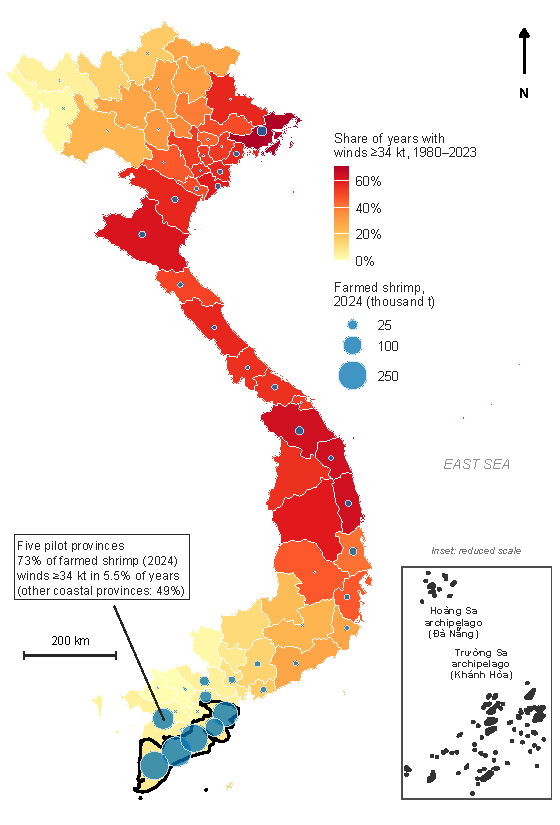
\includegraphics[width=95mm]{jf02_cyclone_shrimp_map.pdf}
\caption{Cyclone hazard and shrimp production by province. Fill: share of years 1980--2023 with modelled winds of at least 34 knots (gale force) anywhere in the province. Circles: farmed shrimp output in 2024 (area proportional to output). Black outline: the five pilot provinces. Inset: the Hoàng Sa (Paracel) and Trường Sa (Spratly) archipelagos, drawn at a reduced scale. Scale bar approximate at 9°N. \textit{Source:} IBTrACS v04 with a modified Rankine wind field; NSO; geoBoundaries; author's calculations.}
\label{fig:map}
\end{figure}

Within the Delta, meteorological hazards vary substantially across 132 districts (Figure~\ref{fig:gis}): from 0 to 101 days per year with maximum temperature above 35°C, longest dry spells of 26 to 68 days, and maximum five-day rainfall of 87 to 211 mm. These indicators are strongly clustered (Moran's $I$ between 0.76 and 0.81, $p<0.001$), and 24--32\% of their variance lies within provinces. A contiguity-constrained SKATER regionalisation \parencite{assuncao2006} with five zones explains 73\% of the multivariate variance, close to the 80\% explained by the 13 provinces, and cuts across five provinces including two pilot provinces. Forty-three of the 44 pilot districts fall into two coastal zones. Meteorological hazards that can be measured from satellites and reanalysis thus vary mainly between provinces; the case for sub-provincial rating rests on salinity and disease, which are not yet mapped.

\begin{figure}[htbp]
\centering
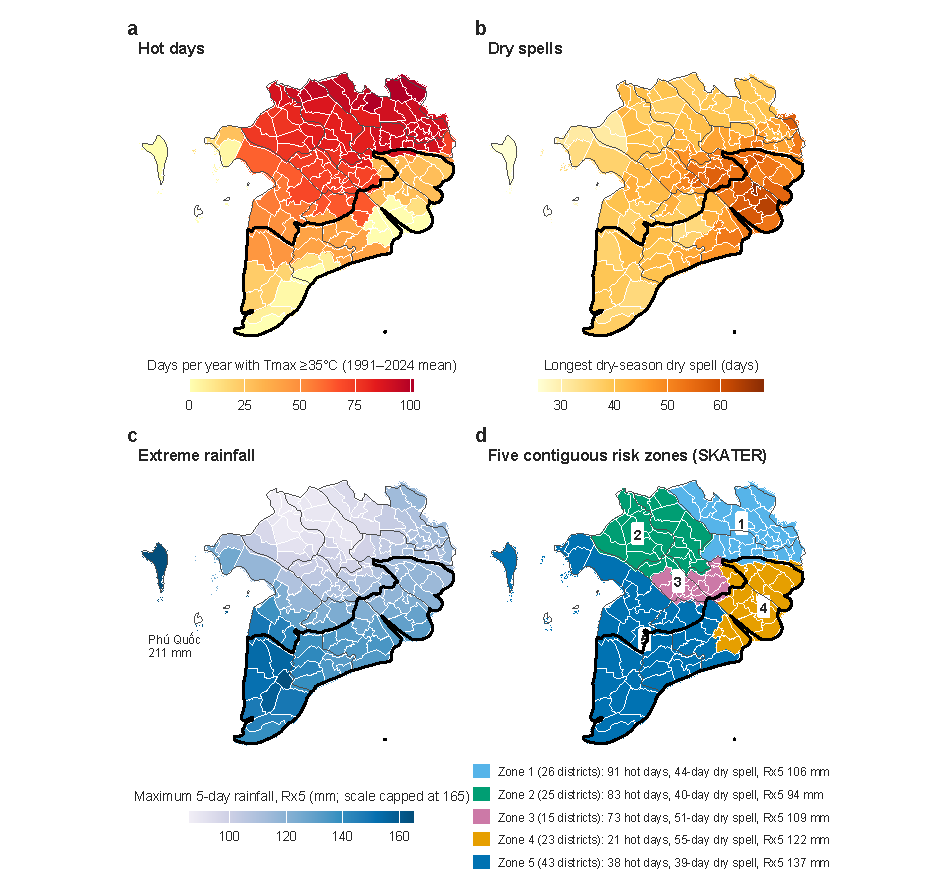
\includegraphics[width=160mm]{jf03_mekong_hazard_zones.pdf}
\caption{District-level meteorological hazards in the 132 Mekong Delta districts, 1991--2024 means. (a) Days per year with maximum temperature of at least 35°C. (b) Longest dry spell in the dry season. (c) Maximum five-day rainfall; the colour scale is capped at the mainland maximum (165 mm) and Phú Quốc island (211 mm) is labelled. (d) Five contiguous risk zones from SKATER regionalisation \parencite{assuncao2006} on four standardised indicators (hot days, dry spell, Rx5 and cyclone probability); the legend gives each zone's mean profile, and zone numbers are printed on the map. Thin grey lines: provinces; thick black line: pilot provinces. \textit{Source:} CHIRPS; NASA POWER (37 districts without a grid cell take the nearest district's value); IBTrACS; geoBoundaries; author's calculations.}
\label{fig:gis}
\end{figure}

\subsection{Are the hazards changing?}

Figure~\ref{fig:clim} asks whether the hazards that gridded indices measure are trending. On land, the 1991--2024 district series show no robust trend. The median district trend in days with maximum temperature of at least 35°C is $-0.4$ days per decade and is positive and significant at the 5\% level in only 4.5\% of districts; the hot-season maximum temperature rises by a median 0.14°C per decade but significantly in only 2\% of districts; and no district shows a significant trend in dry-season (December--April) rainfall. Variation from year to year dominates: ranked by the Delta-wide mean of the minimum SPEI-3, the five driest years were 1997, 2016, 2002, 2024 and 2015. The coastal ocean tells a different story. In the waters within 50 km of the five pilot provinces the sea-surface temperature anomaly rises by 0.30°C per decade, and marine-heatwave days increase from 6.6 a year in 1999--2009 to 53.2 a year in 2015--2024, reaching 142 days in 2024.

\begin{figure}[htbp]
\centering
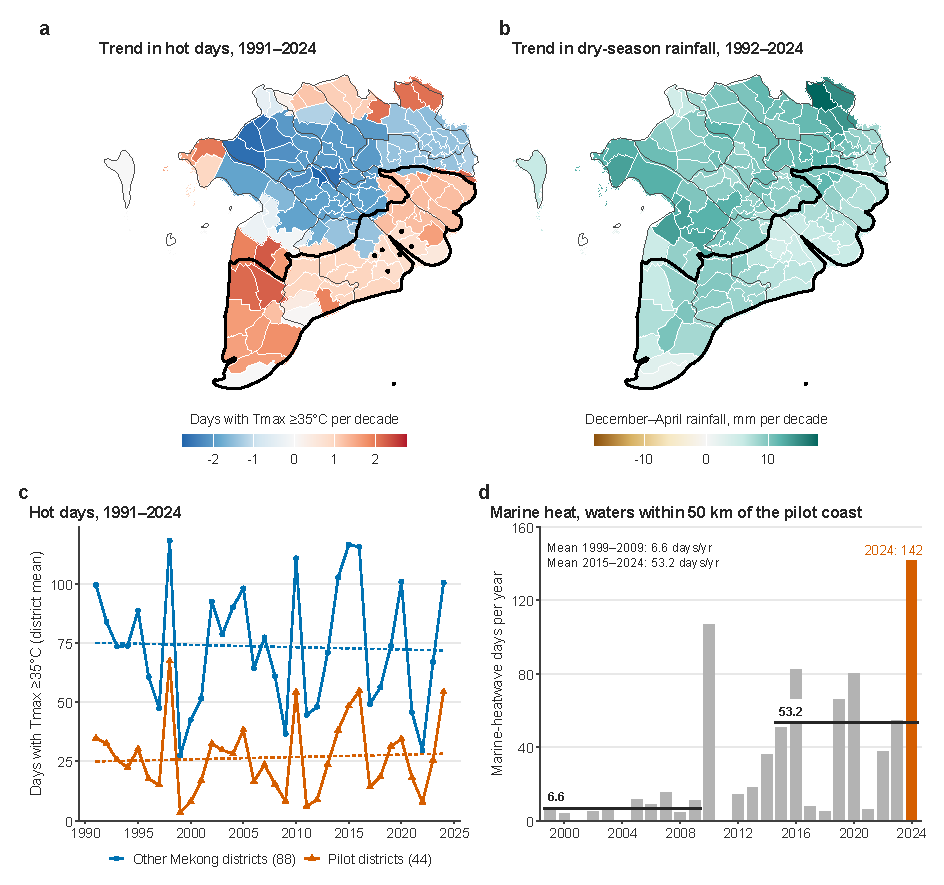
\includegraphics[width=160mm]{jf04_climate_trends.pdf}
\caption{Climate trends in the Mekong Delta. (a) District OLS trend in days with maximum temperature of at least 35°C, 1991--2024. (b) District OLS trend in December--April rainfall, 1992--2024. In (a) and (b) black dots mark districts with $p<0.05$; diverging colour scales follow the IPCC convention (red--blue for temperature, brown--green for precipitation) and are symmetric about zero. (c) Mean annual hot days across pilot (44) and other Mekong (88) districts, with OLS trend lines (dashed). (d) Marine-heatwave days per year in ocean waters within 50 km of the five pilot provinces, 1999--2024, defined as days in spells of at least five days above the 90th percentile of the day-of-year climatology \parencite{hobday2016}; horizontal lines give the 1999--2009 and 2015--2024 means. \textit{Source:} CHIRPS; NASA POWER (37 districts take the nearest district's values); NOAA OISST v2.1 \parencite{huang2021oisst}; author's calculations.}
\label{fig:clim}
\end{figure}

Two cautions apply. Thirty-four years are short for detecting trends in noisy district series, and 37 districts borrow temperature from a neighbour, so the absence of a land trend is not evidence that risk is stable. The marine-heatwave baseline excludes 1992--1998, which raises the threshold slightly if those years were cool. For insurance design the implication is nonetheless direct: for heat in coastal waters, which matters for ponds that take in seawater, recent years are not draws from the 1991--2020 distribution, and premiums or triggers calibrated on that climatology would understate current exposure.

\subsection{The first stage}

Table~\ref{tab:firststage} and Figure~\ref{fig:first} report the share of fish-farming households receiving payments. Three facts stand out. The insurance payout share in the pilot provinces never exceeds 1\% over two decades and does not jump after 2019 or 2022. In 2020, the round with the largest sample, none of 890 fish-farming households in the five provinces received an insurance payout or aquaculture compensation (upper 95\% bound 0.4\%). The 2024 share (7 of 820, 0.9\%, CI 0.4--1.8\%) is no higher than in the core control provinces (5 of 285, 1.8\%). A district-level difference-in-differences on the payout indicator gives $-0.014$ (SE 0.012). Finally, in 2022 state relief reached 19 of 169 fish-farming households in the pilot provinces (11\%) while insurance reached none: when losses occur, the state rather than insurers pays.

\begin{table}[htbp]
\centering\scriptsize
\caption{Fish-farming households receiving insurance payouts, compensation and state relief (VHLSS)}
\label{tab:firststage}
\setlength{\tabcolsep}{3.4pt}
\begin{tabular}{@{}lrrrrrrrrrr@{}}
\toprule
 & 2004 & 2006 & 2008 & 2010 & 2012 & 2014 & 2018 & 2020 & 2022 & 2024 \\
\midrule
\multicolumn{11}{@{}l}{\textit{A. Non-life insurance payout (4D code 108; code 105 in 2004)}} \\
5 pilot provinces & 0/221 & 0/249 & 1/268 & 0/233 & 1/494 & 1/197 & 2/195 & 0/890 & 0/169 & 7/820 \\
4 core controls & 1/190 & 0/166 & 0/147 & 1/115 & 0/225 & 0/117 & 0/112 & 1/364 & 0/63 & 5/285 \\
Rest of Vietnam & 14/1,070 & 7/1,008 & 7/949 & 1/798 & 0/1,669 & 3/630 & 0/662 & 17/2,252 & 3/416 & 15/1,995 \\
\midrule
\multicolumn{11}{@{}l}{\textit{B. Aquaculture compensation or support (4B5T2, from 2018)}} \\
5 pilot provinces & & & & & & & 2/195 & 0/890 & 0/169 & 1/820 \\
4 core controls & & & & & & & 0/112 & 0/364 & 0/63 & 0/285 \\
Rest of Vietnam & & & & & & & 9/662 & 26/2,252 & 2/416 & 6/1,995 \\
\midrule
\multicolumn{11}{@{}l}{\textit{C. State relief for disasters or epidemics (4D code 107)}} \\
5 pilot provinces & & 0/249 & 2/268 & 0/233 & 2/494 & 1/197 & 0/195 & 2/890 & 19/169 & 0/820 \\
4 core controls & & 0/166 & 0/147 & 0/115 & 1/225 & 9/117 & 0/112 & 8/364 & 10/63 & 0/285 \\
Rest of Vietnam & & 24/1,008 & 84/949 & 53/798 & 40/1,669 & 9/630 & 8/662 & 33/2,252 & 7/416 & 12/1,995 \\
\bottomrule
\end{tabular}
\begin{minipage}{\textwidth}\footnotesize
\textit{Notes:} Households with a positive value / fish-farming households in the sample. Code 108 covers all non-life insurance. 4B5T2 pools state support and insurance for aquaculture losses. \textit{Source:} VHLSS; author's calculations.
\end{minipage}
\end{table}

\begin{figure}[htbp]
\centering
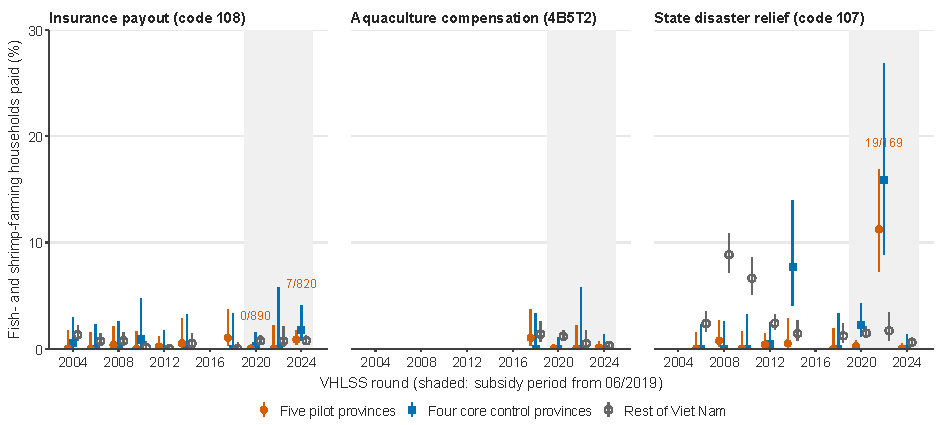
\includegraphics[width=160mm]{jf05_first_stage.pdf}
\caption{The first stage: share of fish- and shrimp-farming households receiving each type of payment, by VHLSS round and province group, unweighted, with Wilson 95\% confidence intervals. Insurance payouts (transfer code 108) cover all non-life insurance; aquaculture compensation (module 4B5T2) exists only from 2018 and pools state support and insurance; state disaster relief is transfer code 107 (from 2006). Shaded: rounds after the shrimp subsidy began in June 2019. Labels give counts for the pilot provinces (households paid / farming households). The four other Mekong provinces are omitted because of small samples. \textit{Source:} VHLSS 2004--2024; author's calculations.}
\label{fig:first}
\end{figure}

\subsection{Programme effects on output}

Table~\ref{tab:did} reports SDID estimates. All are close to zero with confidence intervals that include zero. With the broad donor pool, the estimate for total output is 0.016 (SE 0.066), ruling out effects above roughly 18\%; for shrimp it is 0.110 (SE 0.115), but a placebo that assigns the policy to 2015 gives 0.090, so the gap reflects a pre-existing catch-up rather than the policy. The conventional two-way fixed-effects estimate for shrimp (0.380) is twice its placebo (0.164), illustrating how trend differences bias it. With the eight-province Mekong donor pool the MDE for shrimp exceeds 2 log points, so that design is uninformative. Randomisation inference over the 1,287 possible assignments gives $p=0.96$ for total output. Figure~\ref{fig:sdid}a shows the estimates against their minimum detectable effects.

\begin{table}[htbp]
\centering\footnotesize
\setlength{\tabcolsep}{4pt}
\caption{Programme effect on log provincial output: SDID, placebo and minimum detectable effects, 2005--2024}
\label{tab:did}
\begin{tabular}{@{}llccccc@{}}
\toprule
Outcome & Donor pool & SDID (SE) & Placebo 2015 (SE) & Climate-adj. & MDE & Donors \\
\midrule
Total output & 8 Mekong & $-0.040$ (0.101) & $-0.075$ (0.118) & $-0.084$ & 0.28 & 8 \\
 & Coastal + Mekong & 0.016 (0.066) & $-0.014$ (0.066) & 0.023 & 0.18 & 29 \\
Shrimp & 8 Mekong & 0.405 (0.860) & 0.072 (0.705) & 0.351 & 2.41 & 7 \\
 & Coastal + Mekong & 0.110 (0.115) & 0.090 (0.114) & 0.126 & 0.32 & 23 \\
Fish & 8 Mekong & $-0.123$ (0.151) & $-0.111$ (0.153) & $-0.189$ & 0.42 & 8 \\
 & Coastal + Mekong & $-0.110$ (0.134) & $-0.104$ (0.081) & $-0.125$ & 0.38 & 29 \\
\bottomrule
\end{tabular}
\begin{minipage}{\textwidth}\footnotesize
\textit{Notes:} SDID following \textcite{arkhangelsky2021}; placebo standard errors. Placebo: 2005--2018 sample with treatment assigned to 2015. MDE $=2.8\times$SE. Dropping 2011--2013 and leaving out each pilot province does not change conclusions (shrimp, broad pool: 0.064 to 0.145). \textit{Source:} NSO PX-Web; author's calculations.
\end{minipage}
\end{table}

The event study in Figure~\ref{fig:sdid}b confirms that pre-treatment coefficients are not flat for shrimp and fish: pilot provinces were catching up in shrimp and losing ground in fish well before 2019. Pre-policy balance is also poor at household and district level. Before June 2019 the share of shrimp farmers differs between pilot and control households by 1.37 standard deviations, output value by 1.01, pond area by 0.70 and hot days by $-2.14$. At district level all three control pools are unbalanced (maximum normalised differences 2.15, 1.51 and 1.18), and inverse probability weighting leaves only 3.8 effective control districts. The pilot provinces lie outside the convex hull of potential donors, which \textcite{abadie2021} treats as a precondition for synthetic controls.

\begin{figure}[htbp]
\centering
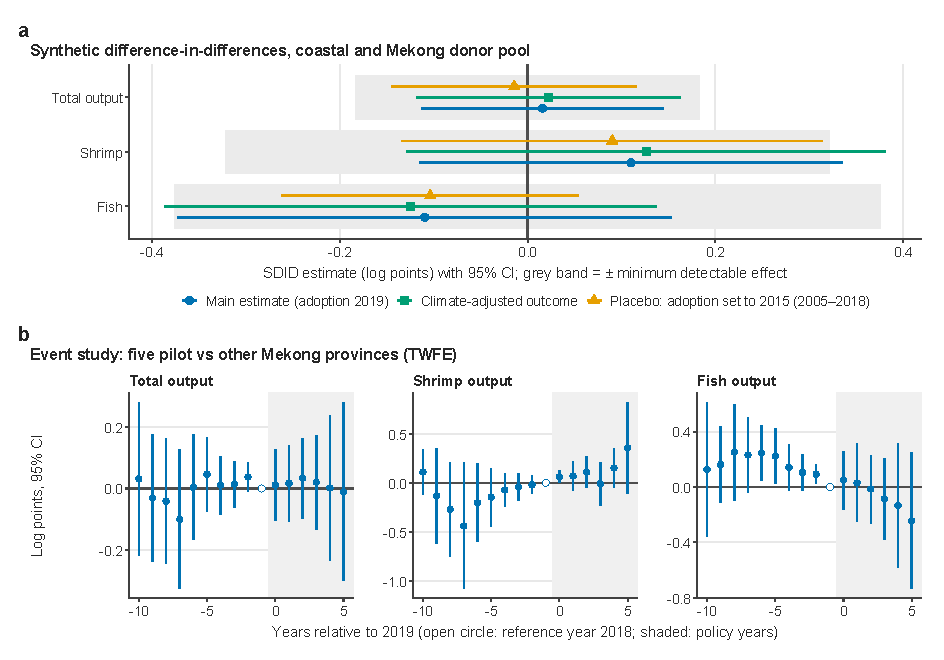
\includegraphics[width=160mm]{jf06_programme_effects.pdf}
\caption{Programme effects on provincial aquaculture output. (a) Synthetic difference-in-differences estimates \parencite{arkhangelsky2021} with other coastal and Mekong provinces as donors (29 for total output and fish, 23 for shrimp): main estimate (adoption in 2019), climate-adjusted outcome, and a placebo that assigns adoption to 2015 on 2005--2018 data; 95\% confidence intervals. Grey bands span $\pm$ the minimum detectable effect ($2.8\times$ the placebo standard error). (b) Two-way fixed-effects event-study coefficients, five pilot provinces versus the eight other Mekong provinces (for shrimp, the four with mean pre-2019 shrimp output of at least 1,000 tonnes), reference year 2018 (open circle); 95\% confidence intervals clustered by province; shaded: policy years. Vertical scales differ across outcomes in (b). \textit{Source:} NSO PX-Web; author's calculations.}
\label{fig:sdid}
\end{figure}

\subsection{Hazards and household output}

Table~\ref{tab:hhfe} reports estimates of equation~\eqref{eq:hh}. No hazard coefficient is significant with commune and province-by-year fixed effects, whether hazards are commune-reported events, annual indices or seasonal indices. The nulls are moderately precise: standard errors of 0.05--0.10 per standard deviation mean that 95\% intervals still include negative effects of 10--25\%. The one exception, extreme rain in July--December for shrimp ($-0.226$, SE 0.106, $p=0.033$) with region-by-year fixed effects, has the predicted sign but shrinks to $-0.079$ (SE 0.137) with province-by-year effects. Among the 47 hazard coefficients estimated across outcomes, samples and fixed-effect structures, this is the only $p$-value below 0.05. After Holm adjustment \parencite{holm1979} the smallest adjusted $p$-value is 1.00, and after Benjamini--Hochberg adjustment \parencite{benjamini1995} the smallest $q$-value is 0.91, so the coefficient is consistent with chance. State relief and exit from aquaculture do not respond to the indices either. Figure~\ref{fig:hh} shows the main coefficients and the distribution of all 47 $p$-values, which lies on or below the line expected if no hazard had any effect.

\begin{figure}[htbp]
\centering
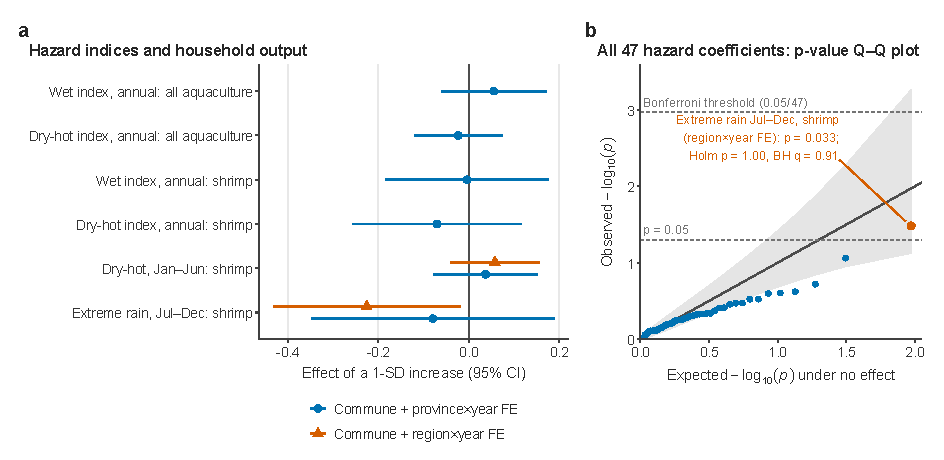
\includegraphics[width=160mm]{jf07_household_hazards.pdf}
\caption{Hazard indices and household aquaculture output. (a) Effect of a one-standard-deviation increase in each index on the inverse hyperbolic sine of output value, with commune fixed effects and province-by-year or region-by-year fixed effects; standard errors clustered by commune; 95\% confidence intervals. (b) Quantile--quantile plot of the $p$-values of all 47 hazard coefficients estimated across outcomes, samples and fixed-effect structures, against the uniform distribution expected under no effect; grey band: pointwise 95\% interval from order statistics. Adjusted values use \textcite{holm1979} and \textcite{benjamini1995}. \textit{Source:} VHLSS 2002--2024; CHIRPS; NASA POWER; IBTrACS; author's calculations.}
\label{fig:hh}
\end{figure}

\begin{table}[htbp]
\centering\footnotesize
\caption{Climate hazards and household aquaculture output (VHLSS, fixed effects)}
\label{tab:hhfe}
\begin{tabular}{@{}llrrr@{}}
\toprule
Outcome, sample, fixed effects & Hazard & Coef. & SE & $N$ \\
\midrule
Farm output; commune + prov.$\times$year & Flood (commune-reported) & $-0.066$ & 0.099 & 6,994 \\
 & Drought (commune-reported) & $-0.042$ & 0.152 & \\
 & Livestock epidemic (commune-reported) & $-0.062$ & 0.071 & \\
Farm output; commune + prov.$\times$year & $H^{wet}$ & 0.055 & 0.059 & 10,442 \\
 & $H^{dry}$ & $-0.023$ & 0.050 & \\
\quad Mekong only & $H^{wet}$ & $-0.031$ & 0.092 & 6,748 \\
 & $H^{dry}$ & $-0.016$ & 0.070 & \\
Shrimp output; commune + prov.$\times$year & $H^{wet}$ & $-0.004$ & 0.092 & 3,637 \\
 & $H^{dry}$ & $-0.071$ & 0.096 & \\
Shrimp, seasonal; commune + reg.$\times$year & $H^{dry}_D$ (matched) & 0.058 & 0.051 & 3,447 \\
 & $H^{wet}_W$ (matched) & $-0.226$ & 0.106 & \\
 & $H^{dry}_W$ (placebo) & $-0.032$ & 0.109 & \\
 & $H^{wet}_D$ (placebo) & 0.048 & 0.067 & \\
\quad same, commune + prov.$\times$year & $H^{wet}_W$ & $-0.079$ & 0.137 & 3,413 \\
Relief (4D-107); commune + prov.$\times$year & $H^{wet}$ & 0.007 & 0.014 & 7,517 \\
 & $H^{dry}$ & $-0.000$ & 0.008 & \\
Exit from aquaculture (panel); prov. + year & $H^{wet}$ & $-0.030$ & 0.038 & 1,200 \\
 & $H^{dry}$ & 0.031 & 0.052 & \\
\bottomrule
\end{tabular}
\begin{minipage}{\textwidth}\footnotesize
\textit{Notes:} Output is the inverse hyperbolic sine of value (million VND). Indices are standardised and measured over the twelve months before the interview. Exit: household farmed in the previous round but not in the current one (2004, 2006, 2008, 2014; 26.7\% exit). Controls: head age, sex, schooling, household size, dependency ratio. SEs clustered by commune. \textit{Source:} VHLSS 2002--2024; CHIRPS; NASA POWER; IBTrACS; author's calculations.
\end{minipage}
\end{table}

Four explanations are compatible with these nulls, and each points to a different next step: the indices miss the risks that matter (salinity, disease and short heat shocks); the VHLSS hides total crop failures because it records only harvested output; province-by-year effects absorb most hazard variation; and climate for 2002--2008 is available only at province level. For policy, the implication is direct: a weather-index product built only from rainfall and temperature, which Decree 346 permits, would carry large basis risk for shrimp farmers \parencite{jensen2016,clarke2016}.

\subsection{Do gridded indices detect local disasters?}

An index product pays when a measured variable crosses a threshold, so its value depends on how closely payouts track the events that cause losses \parencite{clarke2016,jensen2016}. The commune module of the VHLSS offers a direct check: in each round, commune officials report whether floods, storms or droughts occurred in the previous twelve months. For 4,782 commune-rounds in coastal and Mekong provinces (2004--2024), I compute the area under the receiver operating characteristic curve (AUC; \cite{hanley1982}) of each gridded index for the corresponding reported event, both pooled and within province-year. The within-province-year version uses only rounds with district-level climate (2010--2024) and asks whether the index identifies \emph{which} communes are hit in a given province and year, which is what a sub-provincial trigger must do. Intervals come from 499 bootstrap draws of communes.

\begin{figure}[htbp]
\centering
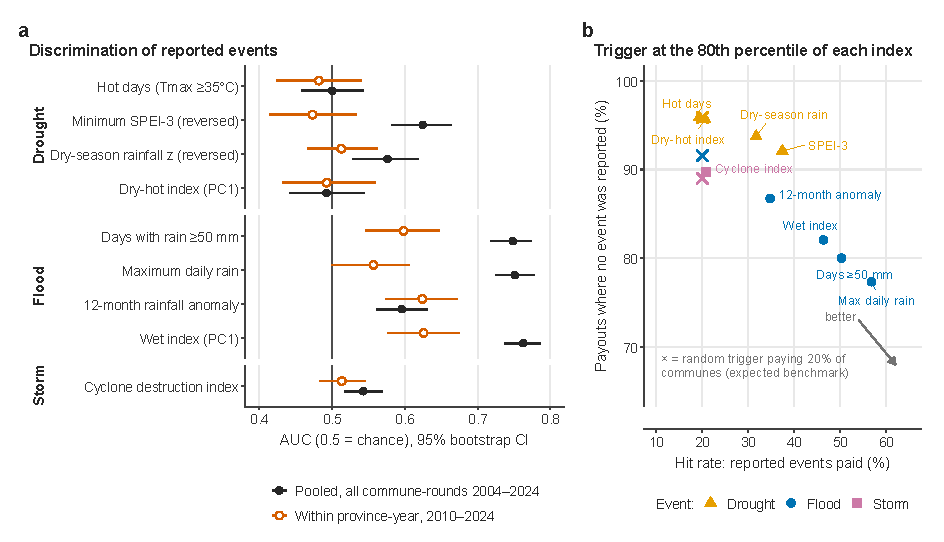
\includegraphics[width=160mm]{jf08_basis_risk.pdf}
\caption{Basis risk: do gridded indices detect the disasters that commune officials report? (a) Area under the ROC curve with 95\% bootstrap intervals (499 draws, resampling communes). Pooled: all commune-rounds 2004--2024. Within province-year: index demeaned by province-year, rounds with district-level climate (2010--2024). 0.5 = no better than chance. (b) Performance of a trigger that pays when an index exceeds its 80th percentile: share of reported events that would be paid (hit rate) against the share of payouts that would go to communes reporting no such event. Crosses mark the expected values for a random trigger that pays 20\% of communes. \textit{Source:} VHLSS commune module; CHIRPS; NASA POWER; IBTrACS; author's calculations.}
\label{fig:auc}
\end{figure}

\begin{table}[htbp]
\centering\footnotesize
\setlength{\tabcolsep}{3.5pt}
\caption{Gridded indices and commune-reported disasters: discrimination and trigger performance}
\label{tab:auc}
\begin{tabular}{@{}llrrccrr@{}}
\toprule
Reported event & Index & $N$ & Events & AUC pooled & AUC within & Hit rate & False payouts \\
\midrule
Drought & Hot days (Tmax $\geq$35°C) & 3,728 & 157 & 0.50 [0.46, 0.54] & 0.48 [0.42, 0.54] & 0.19 & 0.96 \\
 & Minimum SPEI-3 (reversed) & 3,727 & 157 & 0.62 [0.58, 0.66] & 0.47 [0.41, 0.53] & 0.37 & 0.92 \\
 & Dry-season rainfall (reversed) & 4,782 & 190 & 0.58 [0.53, 0.62] & 0.51 [0.47, 0.56] & 0.32 & 0.94 \\
 & Dry-hot index (PC1) & 3,727 & 157 & 0.49 [0.44, 0.54] & 0.49 [0.43, 0.56] & 0.21 & 0.96 \\
\midrule
Flood & Days with rain $\geq$50 mm & 4,782 & 405 & 0.75 [0.72, 0.77] & 0.60 [0.55, 0.65] & 0.50 & 0.80 \\
 & Maximum daily rain & 4,782 & 405 & 0.75 [0.73, 0.78] & 0.56 [0.50, 0.61] & 0.57 & 0.77 \\
 & 12-month rainfall anomaly & 4,782 & 405 & 0.60 [0.56, 0.63] & 0.62 [0.57, 0.67] & 0.35 & 0.87 \\
 & Wet index (PC1) & 4,782 & 405 & 0.76 [0.74, 0.79] & 0.63 [0.58, 0.68] & 0.46 & 0.82 \\
\midrule
Storm & Cyclone destruction index & 4,782 & 526 & 0.54 [0.52, 0.57] & 0.51 [0.48, 0.55] & 0.21 & 0.90 \\
\bottomrule
\end{tabular}
\begin{minipage}{\textwidth}\footnotesize
\textit{Notes:} Unit: commune-round, coastal and Mekong provinces, 2004--2024 (rounds with a commune module). AUC within: index minus its province-year mean, rounds 2010--2024. 95\% intervals from 499 bootstrap draws of communes. Hit rate: share of communes reporting the event in which a trigger at the 80th percentile of the index would pay (a random trigger pays 0.20). False payouts: share of triggered commune-rounds that report no such event. \textit{Source:} VHLSS; CHIRPS; NASA POWER; IBTrACS; author's calculations.
\end{minipage}
\end{table}

Figure~\ref{fig:auc} and Table~\ref{tab:auc} show the results. Rainfall indices separate flooded from non-flooded communes reasonably well when pooled (AUC 0.75--0.76 for heavy-rain days, maximum daily rain and the wet index), but much of this power comes from distinguishing wet provinces and years; within province-year the AUC falls to 0.56--0.63. Drought is barely detected: the best index, the minimum SPEI-3, has a pooled AUC of 0.62 and a within-province-year AUC of 0.47, and the heat and dry-hot indices are no better than chance in either version. The cyclone index barely separates communes reporting storms (0.54). A trigger set at the 80th percentile of each index, paying in one commune-year in five, would pay in 19--37\% of communes that report a drought, close to the 20\% of a random trigger, and in 35--57\% of those that report a flood; between 77\% and 96\% of its payouts would go to communes that report no such event. Commune reports are themselves noisy and record events rather than farm losses, so these figures bound rather than measure basis risk. They reinforce the household results: at the resolution now available, gridded meteorological indices do not capture the local disasters that officials record, least of all drought.

\subsection{Pricing}

Table~\ref{tab:premium} reports illustrative premiums for the provincial yield-index product. Raw pure premium rates range from 0 to 6.6\% across provinces, but most of this dispersion is sampling noise. With only 20 annual observations per province, the Bühlmann--Straub credibility factor is 0.59 in the Mekong Delta ($k = 13.7$) and 0.29 among other coastal provinces ($k = 48.8$). Zero or very low raw rates for Bạc Liêu and Cà Mau reflect smoothed provincial totals, not low farm-level risk: Bạc Liêu's output rose every year from 2005 to 2024. The pooled generalised Pareto tail has shape $\hat\xi = 0.016$ with a bootstrap 95\% interval of $[-0.47, 0.27]$, so the data cannot distinguish thin from heavy tails. Tail loadings must therefore come from long hazard series combined with damage functions, not from short output series. Figure~\ref{fig:prem} shows how far credibility weighting pulls each provincial rate towards its regional mean.

\begin{figure}[htbp]
\centering
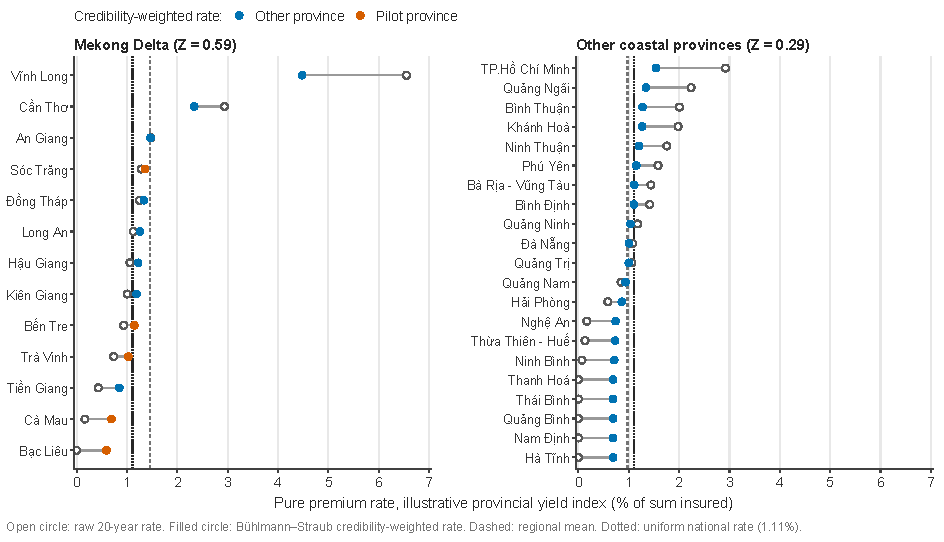
\includegraphics[width=160mm]{jf09_premium_credibility.pdf}
\caption{Raw and credibility-weighted pure premium rates for an illustrative provincial yield-index product, 34 coastal and Mekong provinces. Open circles: raw rates from 20 years of output shortfalls (payout $=\max(0,0.9-Q/\hat Q)$ with a leave-one-out quadratic trend). Filled circles: Bühlmann--Straub credibility-weighted rates \parencite{buhlmann2005}, with credibility factors $Z=0.59$ (Mekong Delta) and $0.29$ (other coastal provinces). Dashed lines: regional means; dotted line: output-weighted uniform rate (1.11\%). Shortfalls include disease and price effects, so these are not disaster-insurance tariffs. \textit{Source:} NSO; author's calculations.}
\label{fig:prem}
\end{figure}

\begin{table}[htbp]
\centering\small
\caption{Illustrative provincial yield-index premiums: raw, tail-loaded and credibility-weighted (\% of sum insured)}
\label{tab:premium}
\begin{tabular}{@{}lcccccc@{}}
\toprule
Province & Raw PPR & Payout years & CVaR$_{95}$ & Loaded & Credibility PPR & Cred.\ loaded \\
\midrule
Bạc Liêu & 0.00 & 0/20 & 0.0 & 0.00 & 0.59 & 0.59 \\
Bến Tre & 0.94 & 2/20 & 13.7 & 2.21 & 1.15 & 2.42 \\
Cà Mau & 0.16 & 1/20 & 3.3 & 0.48 & 0.69 & 1.00 \\
Sóc Trăng & 1.29 & 4/20 & 17.7 & 2.93 & 1.36 & 3.00 \\
Trà Vinh & 0.74 & 2/20 & 9.7 & 1.63 & 1.03 & 1.92 \\
\midrule
Vĩnh Long (highest) & 6.55 & 8/20 & 48.7 & 10.76 & 4.48 & 8.69 \\
\midrule
Uniform rate (34 provinces) & 1.11 & & & 2.10 & & \\
\bottomrule
\end{tabular}
\begin{minipage}{\textwidth}\footnotesize
\textit{Notes:} Payout $=\max(0,0.9-Q/\hat Q)$ with a leave-one-out quadratic trend. Loading $=0.10\times(\mathrm{CVaR}_{95}-\mathrm{PPR})$, CVaR computed exactly on 20 years. Credibility: $Z=0.593$ (Mekong) and $0.291$ (other coastal). The uniform rate is weighted by 2024 output. Shortfalls include disease and price effects, so these are not disaster-insurance tariffs. \textit{Source:} NSO; author's calculations.
\end{minipage}
\end{table}

\subsection{Simulated designs}

Table~\ref{tab:sim} and Figure~\ref{fig:scen} summarise the equilibrium simulation. Parameters are assumed, so the results are informative about rankings, not levels. Provincial rating barely reduces adverse selection: non-poor take-up rises only from 40.8\% to 41.3\%, because provincial differences in systemic risk are small relative to private risk differences. Zone rating with a map that correlates 0.8 with true risk raises non-poor take-up to 54.1\% at a lower subsidy per household. Raising the subsidy for non-poor households from 20\% to 50\%, as Decree 346 allows, raises their take-up to 65.0\% but increases subsidy cost per household by 40\% and leaves adverse selection in place; combining both instruments gives the highest coverage (81.1\%).

\begin{table}[htbp]
\centering\small
\caption{Simulated market equilibrium by information structure and subsidy schedule (assumed parameters)}
\label{tab:sim}
\begin{tabular}{@{}lcccccc@{}}
\toprule
Design & \multicolumn{3}{c}{Take-up (\%)} & Selection & Subsidy/hh & $\sum\Delta CE$/ \\
\cmidrule(lr){2-4}
 & All & Poor & Non-poor & index & (\% wealth) & subsidy \\
\midrule
\multicolumn{7}{@{}l}{\textit{A. Current subsidies 90\%/20\%}} \\
Uniform premium & 56.3 & 93.3 & 40.8 & 1.39 & 0.96 & 1.13 \\
Provincial premium & 56.9 & 93.9 & 41.3 & 1.37 & 0.95 & 1.13 \\
Zone premium, $\rho=0.5$ & 60.8 & 95.5 & 46.3 & 1.31 & 0.93 & 1.14 \\
Zone premium, $\rho=0.8$ & 66.7 & 97.0 & 54.1 & 1.23 & 0.91 & 1.15 \\
Zone premium, $\rho=0.95$ & 73.9 & 98.1 & 63.7 & 1.16 & 0.88 & 1.17 \\
Full information & 99.2 & 99.2 & 99.2 & 1.01 & 0.90 & 1.18 \\
\midrule
\multicolumn{7}{@{}l}{\textit{B. Subsidies 90\%/50\% (Decree 346/2026 range)}} \\
Uniform premium & 73.6 & 94.0 & 65.0 & 1.25 & 1.35 & 1.11 \\
Zone premium, $\rho=0.8$ & 85.9 & 97.2 & 81.1 & 1.12 & 1.37 & 1.12 \\
\bottomrule
\end{tabular}
\begin{minipage}{\textwidth}\footnotesize
\textit{Notes:} 6,000 households allocated to 34 provinces by 2024 output; private loss probability Beta(1.2, 8), severity Beta(2, 5); indemnity contract with 10\% deductible; CRRA $\gamma\sim U(1,3)$; loading 25\%; 30\% poor households; no relief, trigger rule or disease. Selection index: mean expected loss of buyers over that of all households. \textit{Source:} author's simulation.
\end{minipage}
\end{table}

\begin{figure}[htbp]
\centering
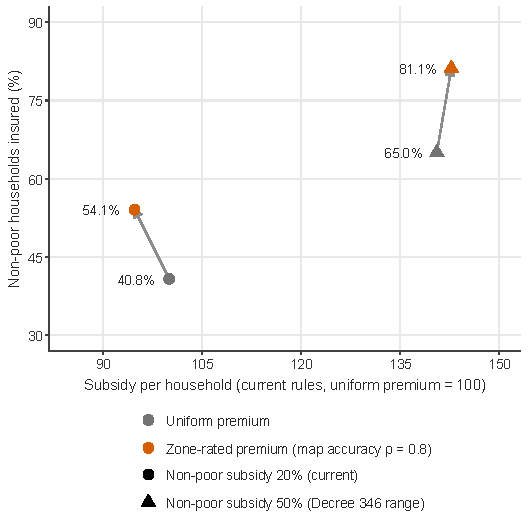
\includegraphics[width=90mm]{jf10_policy_scenarios.pdf}
\caption{Simulated take-up among non-poor households and subsidy cost per household under four designs; arrows show the move from a uniform to a zone-rated premium at each subsidy level. Subsidy cost is indexed to current rules with a uniform premium (= 100). All parameters are assumed (see Table~\ref{tab:sim}); the figure ranks designs and does not forecast take-up. \textit{Source:} author's simulation.}
\label{fig:scen}
\end{figure}

A caution follows directly from the first-stage evidence. The simulation predicts take-up of about 56\% under current rules; observed take-up is near zero. The gap shows that constraints absent from the model, namely the declaration-based trigger, the disease exclusion and insurers' failure to offer the product, dominate adverse selection in practice. The simulation should therefore be read as a ranking of pricing designs conditional on a product being offered, not as a forecast of take-up.

%====================================================================
\section{Discussion}
\label{sec:discussion}

\subsection{Why coverage is near zero: ranking the explanations}

The evidence allows a tentative ranking. \textit{Supply-side retreat} is supported by the 2011--2013 experience (claims of about 3.1 times premiums, reinsurers declining shrimp risk) and by the absence of any shrimp province among implementing localities after 2019. \textit{Trigger and scope design} is supported by the legal text: chronic hazards such as salinity are listed but rarely ``announced'' at the scale of individual ponds, and disease, which household surveys identify as the most frequent risk \parencite{kiet2021ruiro,joffre2018}, is excluded. \textit{Charity hazard} is consistent with the 2022 pattern, when relief reached 11\% of pilot households and insurance none, but the VHLSS cannot identify crowding out, and whether Decree 02/2017 nets insurance indemnities against relief remains to be verified. \textit{Adverse selection under uniform pricing} is theoretically relevant and is the focus of the pricing analysis, but it cannot explain zero coverage on its own. Stated-preference studies show latent demand when products fit farmers' needs \parencite{nguyenkat2021,tu2025}, which argues against a pure lack of demand.

\subsection{Limitations}

Seven limitations qualify these conclusions. First, the VHLSS records receipt of payments rather than participation, and receipt can be low simply because few insured events occurred in the recall window. Second, salinity and disease are not observed. Third, provincial estimates erase pond-level risk, and household estimates rely on limited within-province hazard variation. Fourth, administrative figures come from press reports and are not fully consistent across sources. Fifth, commune disaster reports are a noisy benchmark: officials may under-report slow-onset drought or over-report events that attract relief, which biases the AUC toward 0.5 in the first case and in an unknown direction in the second. Sixth, I considered satellite night-time lights (NASA Black Marble) as an independent outcome but did not use them: pond aquaculture in the Delta is largely unlit at the 500 m resolution of VIIRS, so most rural pixels record zero radiance; radiance tracks towns and industry rather than farm output \parencite{henderson2012,roman2018}; the series starts in 2012, leaving a short pre-period; and with a near-zero first stage there is no programme effect for lights to detect. Their established use, local damage from acute shocks such as typhoons \parencite{elliott2015}, does not match the slow-onset hazards studied here. Seventh, the contents of Decision 13/2022 and Decree 346/2026 were verified through secondary sources; transitional provisions remain to be checked against the original texts. VHLSS microdata after 2010 are restricted, so replication requires a licence; code and metadata are available.

%====================================================================
\section{Policy implications}
\label{sec:policy}

The evidence suggests that the binding constraints lie in design, data and supply rather than in the subsidy rate. Four implications follow, ordered by the strength of the evidence.

\begin{enumerate}
\item \textbf{Replace declaration-based triggers with objective thresholds} for salinity and heat (station salinity, air and coastal-water temperature indices, water levels), calibrated on recent years rather than on 1991--2020 climatologies given the rise in marine heat when provincial People's Councils adopt resolutions under Decree 346. This addresses the administrative basis risk in equation~\eqref{eq:trigger}.
\item \textbf{Publish programme data} (participants, area, premiums, indemnities by commune, year and species) and loss data by cause. Without them, neither insurers nor government can price or evaluate the programme.
\item \textbf{Build a commune-level risk map as a public good}, combining hazards, exposure from the national aquaculture database \parencite{mae2026qd2120} and vulnerability, and use it for three to five premium zones with progressive subsidies applied to risk-based premiums and caps for poor households in high-risk zones \parencite{shirai2026drf,aguilar2018fao}.
\item \textbf{Pilot index products with evaluation}, using multiscale designs to limit basis risk \parencite{elabed2013}, and measure basis risk against indemnity data before scaling; the commune-level test used here shows that rainfall and temperature indices at current resolution would miss most local droughts. Disease requires a separate mechanism tied to biosecurity.
\end{enumerate}

Raising subsidies under Decree 346 without these changes risks spending more on a product that farmers do not buy and insurers do not sell.

%====================================================================
\section{Conclusion}
\label{sec:conclusion}

Vietnam's subsidised shrimp insurance has, on the evidence of two decades of nationally representative survey data and of administrative statements, almost never reached farmers. The legal peril list already covers the Delta's main climate hazards; the contract pays only after official declarations, excludes disease, and has not been offered by insurers since a loss-making pilot. Province-level programme evaluation can only bound the effect of a policy that was barely implemented, and gridded weather indices track neither household losses nor the local disasters that officials report, while heat in the coastal waters that feed shrimp ponds is rising faster than the historical record implies. The next stage of research should obtain administrative participation and claims data, observed salinity and disease records, and evidence from insurers, so that the trigger probability $\phi$ and the unlisted loss share in equation~\eqref{eq:trigger} can be estimated directly.

\clearpage
\printbibliography[title={References}]

%====================================================================
\clearpage
\appendix
\section*{Appendix}
\addcontentsline{toc}{section}{Appendix}
\renewcommand{\thetable}{A\arabic{table}}
\setcounter{table}{0}

\begin{table}[htbp]
\centering\scriptsize
\caption{Cyclone exposure and log provincial output (two-way fixed effects, 2005--2023)}
\label{tab:twfe}
\begin{tabular}{@{}llcccccccc@{}}
\toprule
Model & Variable & Coef. & SE (CR1) & $p_{\text{CR1}}$ & SE (DK) & $p_{\text{DK}}$ & $p_{\text{WCR}}$ & $N$ & Provinces \\
\midrule
(1) Total output & $DI_t$ & $-0.159$ & 0.294 & 0.593 & 0.173 & 0.360 & 0.601 & 646 & 34 \\
 & $DI_{t-1}$ & $-0.161$ & 0.396 & 0.688 & 0.270 & 0.552 & 0.734 & & \\
(3) Shrimp & $DI_t$ & $-0.531$ & 0.399 & 0.193 & 0.252 & 0.035 & 0.227 & 579 & 32 \\
 & $DI_{t-1}$ & $-0.823$ & 0.553 & 0.147 & 0.282 & 0.004 & 0.178 & & \\
(4) Shrimp, placebo & $DI_{t+1}$ & $-0.066$ & 0.602 & 0.913 & 0.572 & 0.908 & 0.923 & 549 & 32 \\
(5) Shrimp, excl.\ Mekong & $DI_t$ & $-0.654$ & 0.435 & 0.148 & 0.284 & 0.021 & 0.160 & 393 & 21 \\
 & $DI_{t-1}$ & $-0.921$ & 0.602 & 0.142 & 0.305 & 0.003 & 0.204 & & \\
(6) Fish & $DI_t$ & $-0.122$ & 0.216 & 0.574 & 0.118 & 0.299 & 0.587 & 646 & 34 \\
(7) EM-DAT counts & Storms & $-0.023$ & 0.016 & 0.169 & 0.012 & 0.066 & 0.172 & 612 & 34 \\
 & Droughts & $-0.023$ & 0.036 & 0.533 & 0.059 & 0.700 & 0.521 & & \\
\bottomrule
\end{tabular}
\begin{minipage}{\textwidth}\footnotesize
\textit{Notes:} Province and year fixed effects. $DI$ is a cubic destruction index (one unit = 100-kt winds over the whole province). CR1: province-clustered SEs. DK: Driscoll--Kraay (2 lags). WCR: restricted wild cluster bootstrap-$t$, 999 replications, Rademacher weights \parencite{cameron2008,driscoll1998}. \textit{Source:} NSO; IBTrACS; EM-DAT; author's calculations.
\end{minipage}
\end{table}

\paragraph{Data and code availability.} Provincial output data (NSO PX-Web), IBTrACS, CHIRPS, NASA POWER and OISST are public. VHLSS microdata are available from the National Statistics Office under licence. The R code that harmonises the survey, builds the hazard measures, and produces every table and figure, together with a log of each step and checksums of all raw inputs, is available from the author.

\end{document}
